\chapter{Background \& Objectives}

This section should discuss your preparation for the project, including background reading, your analysis of the problem and the process or method you have followed to help structure your work.  It is likely that you will reuse part of your outline project specification, but at this point in the project you should have more to talk about. 

\textbf{Note}: 

\begin{itemize}
   \item All of the sections and text in this example are for illustration purposes. The main Chapters are a good starting point, but the content and actual sections that you include are likely to be different.
   
   \item Look at the document on the Structure of the Final Report for additional guidance. 
   
\end {itemize}

\section{Background}
What was your background preparation for the project? What similar systems did you assess? What was your motivation and interest in this project? 

%we looked mostly at zegami and the access-phenomics site, these were the similar systems that we researched primarily

\section{Analysis}
Taking into account the problem and what you learned from the background work, what was your analysis of the problem? How did your analysis help to decompose the problem into the main tasks that you would undertake? Were there alternative approaches? Why did you choose one approach compared to the alternatives? 

There should be a clear statement of the objectives of the work, which you will evaluate at the end of the work. 

In most cases, the agreed objectives or requirements will be the result of a compromise between what would ideally have been produced and what was felt to be possible in the time available. A discussion of the process of arriving at the final list is usually appropriate.

\section{Process}

Plan driven approaches traditionally associated with software development projects usually expect that all system requirements are understood and collected prior to any further work on design or implementation. A number of factors made such an approach unsuitable for this project, chiefly a lack of domain knowledge made up-front requirement gathering difficult and the requirements themselves were likely to be poorly defined and subject to change. 

The methodology used for the delivery of the project was an agile approach based on the popular SCRUM methodology. For the duration of the project, work would be carried out in time-boxed iterations or `sprints', each a week long. Sprints would begin with a planning session and end with a release of the system software. At the conclusion of each sprint a short retrospective analysis of the sprint would take place, looking at what went well and what could improve for the next iteration. The focus on incremental delivery of working software allowed to project to evolve in an emergent fashion whilst remaining continuously functional as features were prototyped, designed and implemented.  

System requirements were broken down into user stories which in turn were broken down into individual tasks if necessary. As in SCRUM, these stories were held in a backlog until being added into a current or future sprint depending on priority and the goal for a particular sprint. Emergent issues such as priority bugs could easily be incorporated into the wider context of the current sprint if necessary which allowed work to be focused on the most pressing issues. The Jira \cite{jira} issue tracking application was used in support of this process providing an environemnt in which to specify and track user stories,task and sprints, see section~\ref{jira_sec} for further details. 

During a sprint, each day would begin with a quick overview of tasks in the sprint, replicating the `stand-up' meetings common in SCRUM. Work would be commenced or continued on the task deemed highest priority at the time. At the end of each day a short update would often be posted on the project blog available at \url{https://siongriffithsblog.wordpress.com/} summarising the days activity. The blog itself has proven to be a useful part of the process, helping to document certain aspects of the implementation and design that may have otherwise been forgotten.


\subsection{Time Management}
Effective management of time is a key consideration of any reasonable development process model. Partway through the project it was decided to fully adopt the Pomodoro technique \cite{pomodoro}, working in blocks of twenty five minutes with complete focus on the task at hand, referred to as Pomodoros. A five minute break is taken after each successful twenty five minute work block in order to avoid the mental fatigue of attempting to remain focused and productive for an extended amount of time. Taking these regular, short breaks allowed for a higher degree of productivity over the course of a work day.

Having distinct blocks of time in which to complete work compliments the SCRUM approach to effort tracking and estimation. Although not part of the initial process, towards the latter half of the project after gaining a sufficient feel for the possible output of a single Pomodoro, all work was estimated in terms of the Pomodoros required to complete the task. The goal for a given sprint was to achieve sixty Pomodoro and use this figure as the budget for work that could be done. It was fairly difficult to estimate in terms of Pomodoro and often fairly inaccurate, although the productivity aspect certainly works, the more abstract and popular `story-point' method of effort estimation is what would be used if the project was repeated.

Figure ~\ref{fig:pomo1} shows the early Pomodoro tracking during two iterations. It was preferable to have Pomodoro goals for a given sprint rather than concrete work times (for example nine-to-five) since this allowed a great deal of flexibility whilst also maintaining that a weeks worth of work was to be done.  

\begin{figure}[H]
    \centering
    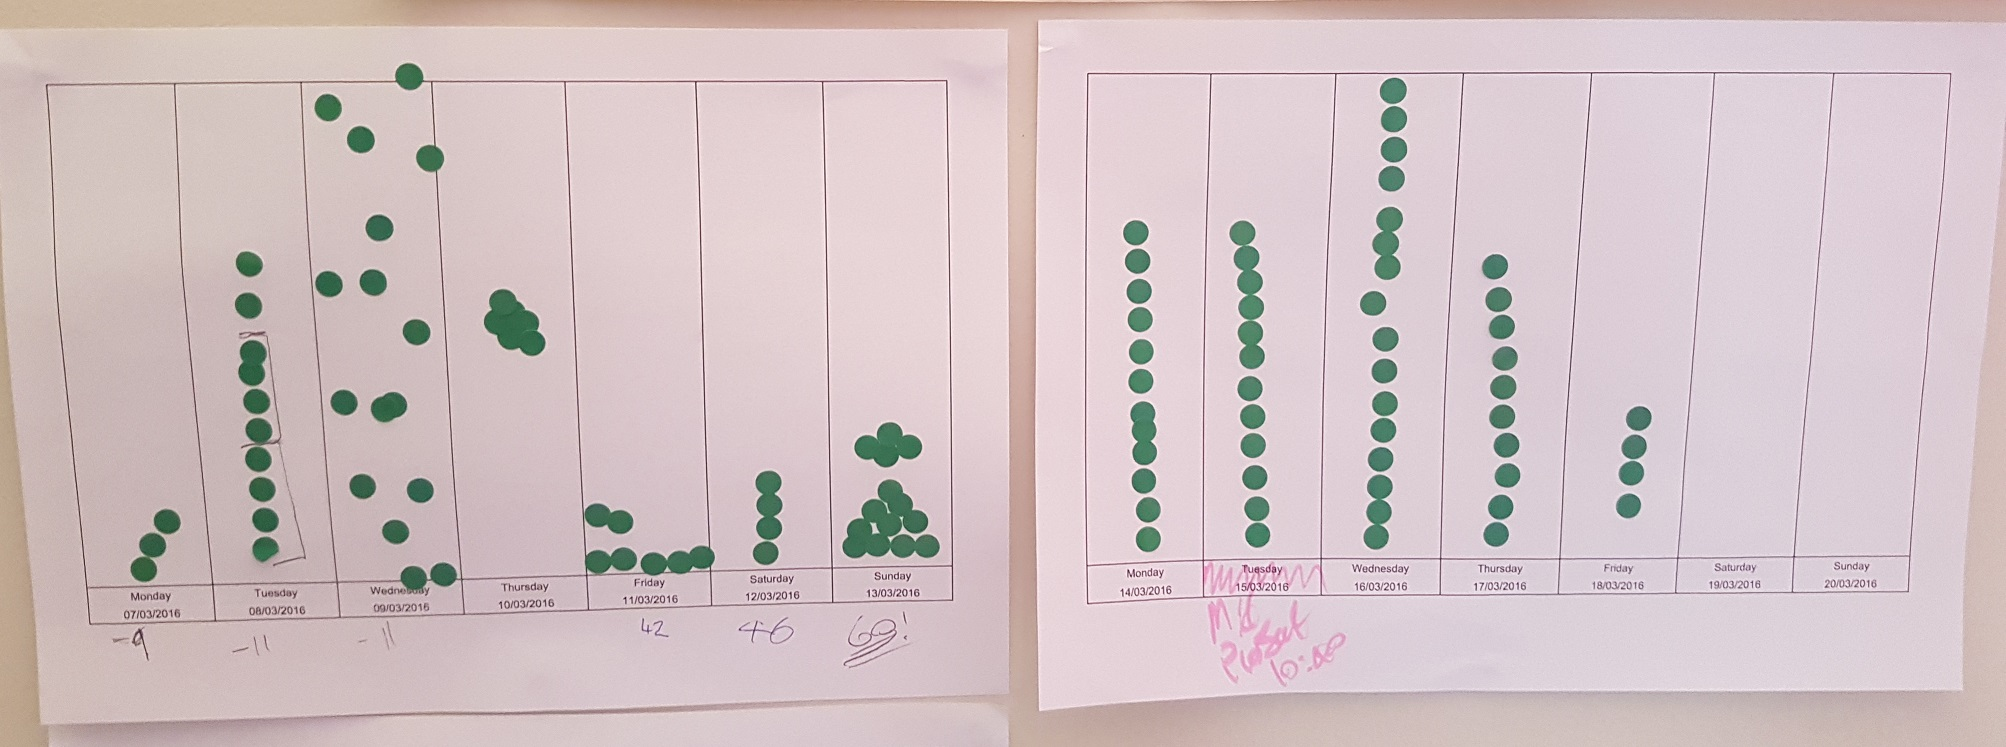
\includegraphics[width=\textwidth]{images/process/pomotrack}
    \caption{Tracking pomodoros}
    \label{fig:pomo1}
\end{figure}


%The process used for the project was an agile based approach similar in style to Scrum although adapted for a project team of one. The process centred around User Stories and short iterations of one week. 

